\chapter{Mécanismes de sécurité et mise en production}

\section{Intégrer le transcodage des clés}

\chapter{Mise en production}

\section{Configuration et installation générale}

\subsection{Configuration du serveur web}

\subsection{Nettoyage de l'application et contrôles à réaliser}

\subsection{Installation de la base de données des droits}

\subsection{Nettoyage des comptes par défaut}

\section{Travailler avec plusieurs applications différentes à partir du même code}\label{dnsmultiple}

Dans certains cas, l'application réalisée doit permettre de travailler avec des bases de données différentes selon le contexte, pour éviter de mélanger les informations. La première solution consiste à créer autant de copies que nécessaire du logiciel.

La seconde consiste à n'utiliser qu'un seul code, mais en paramétrant les informations spécifiques à chaque base de données.

Voici le principe général (\textit{cf.} schéma \ref{dnsmultipleschema})  :
\begin{figure}[th]
\label{dnsmultipleschema}
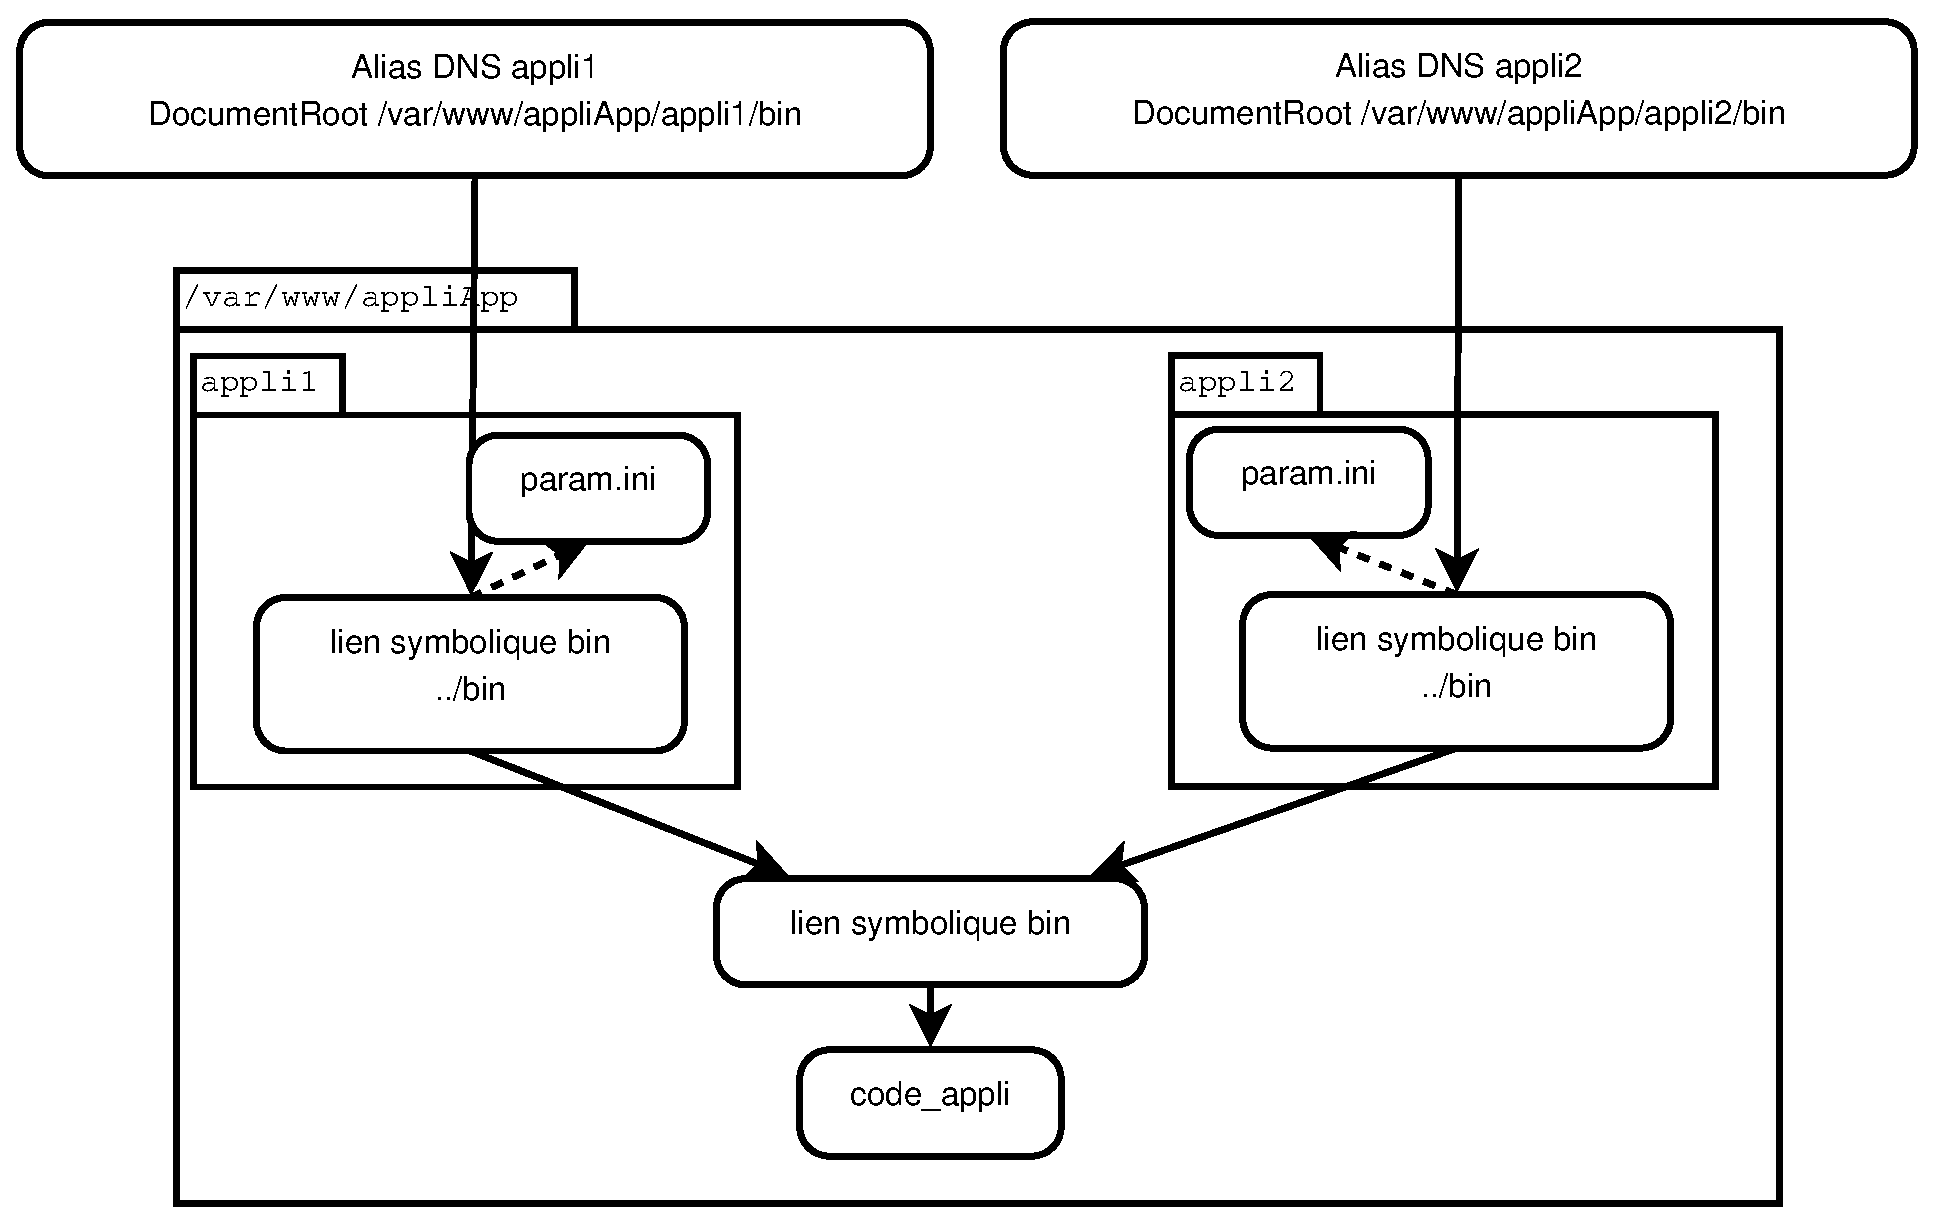
\includegraphics[width=\linewidth]{dessin/dnsmultiple}
\caption{Schéma général d'implémentation pour utiliser le même code avec des noms d'application et des jeux de données différents}
\end{figure}

Dans le paramétrage de l'alias DNS (en principe, dans \textbf{/etc/apache2/sites-available}), l'application pointe vers le dossier \textbf{/var/www/appliApp/appli1/bin}. 
\textit{/var/www} correspond à la racine du site web, \textit{appliApp} au dossier racine de l'application, \textit{appli1} au dossier spécifique de l'alias DNS.

Ce dossier \textit{appli1} ne contient que deux fichiers : \textbf{param.ini}, qui contient les paramètres spécifiques, et \textbf{bin}, qui est un lien symbolique vers le dossier \textbf{../bin}. 

Le dossier \textit{../bin} (donc, dans \textit{/var/www/appliApp}) est lui aussi un alias qui pointe vers le code réel de l'application, ici \textbf{code\_appli}.

Le fichier \textbf{param.inc.php} décrit l'entrée suivante :
\begin{lstlisting}
$paramIniFile = "../param.ini";
\end{lstlisting}

Le fichier \textbf{param.ini} sera cherché dans le dossier parent du code de l'application, c'est à dire soit dans \textit{appli1}, soit dans \textit{appli2} dans cet exemple.

Il suffit qu'il contienne les paramètres adéquats pour rendre l'application utilisable dans des contextes différents à partir du même code initial.